% Figure reproduced from Butler and Butler (2026), "Legal RAG Bench: An End-to-End
% Benchmark for Legal RAG", Figure 1, for scholarly discussion and critique within this
% review. Copyright remains with the original authors/publisher.
\begin{figure*}[t]
\centering
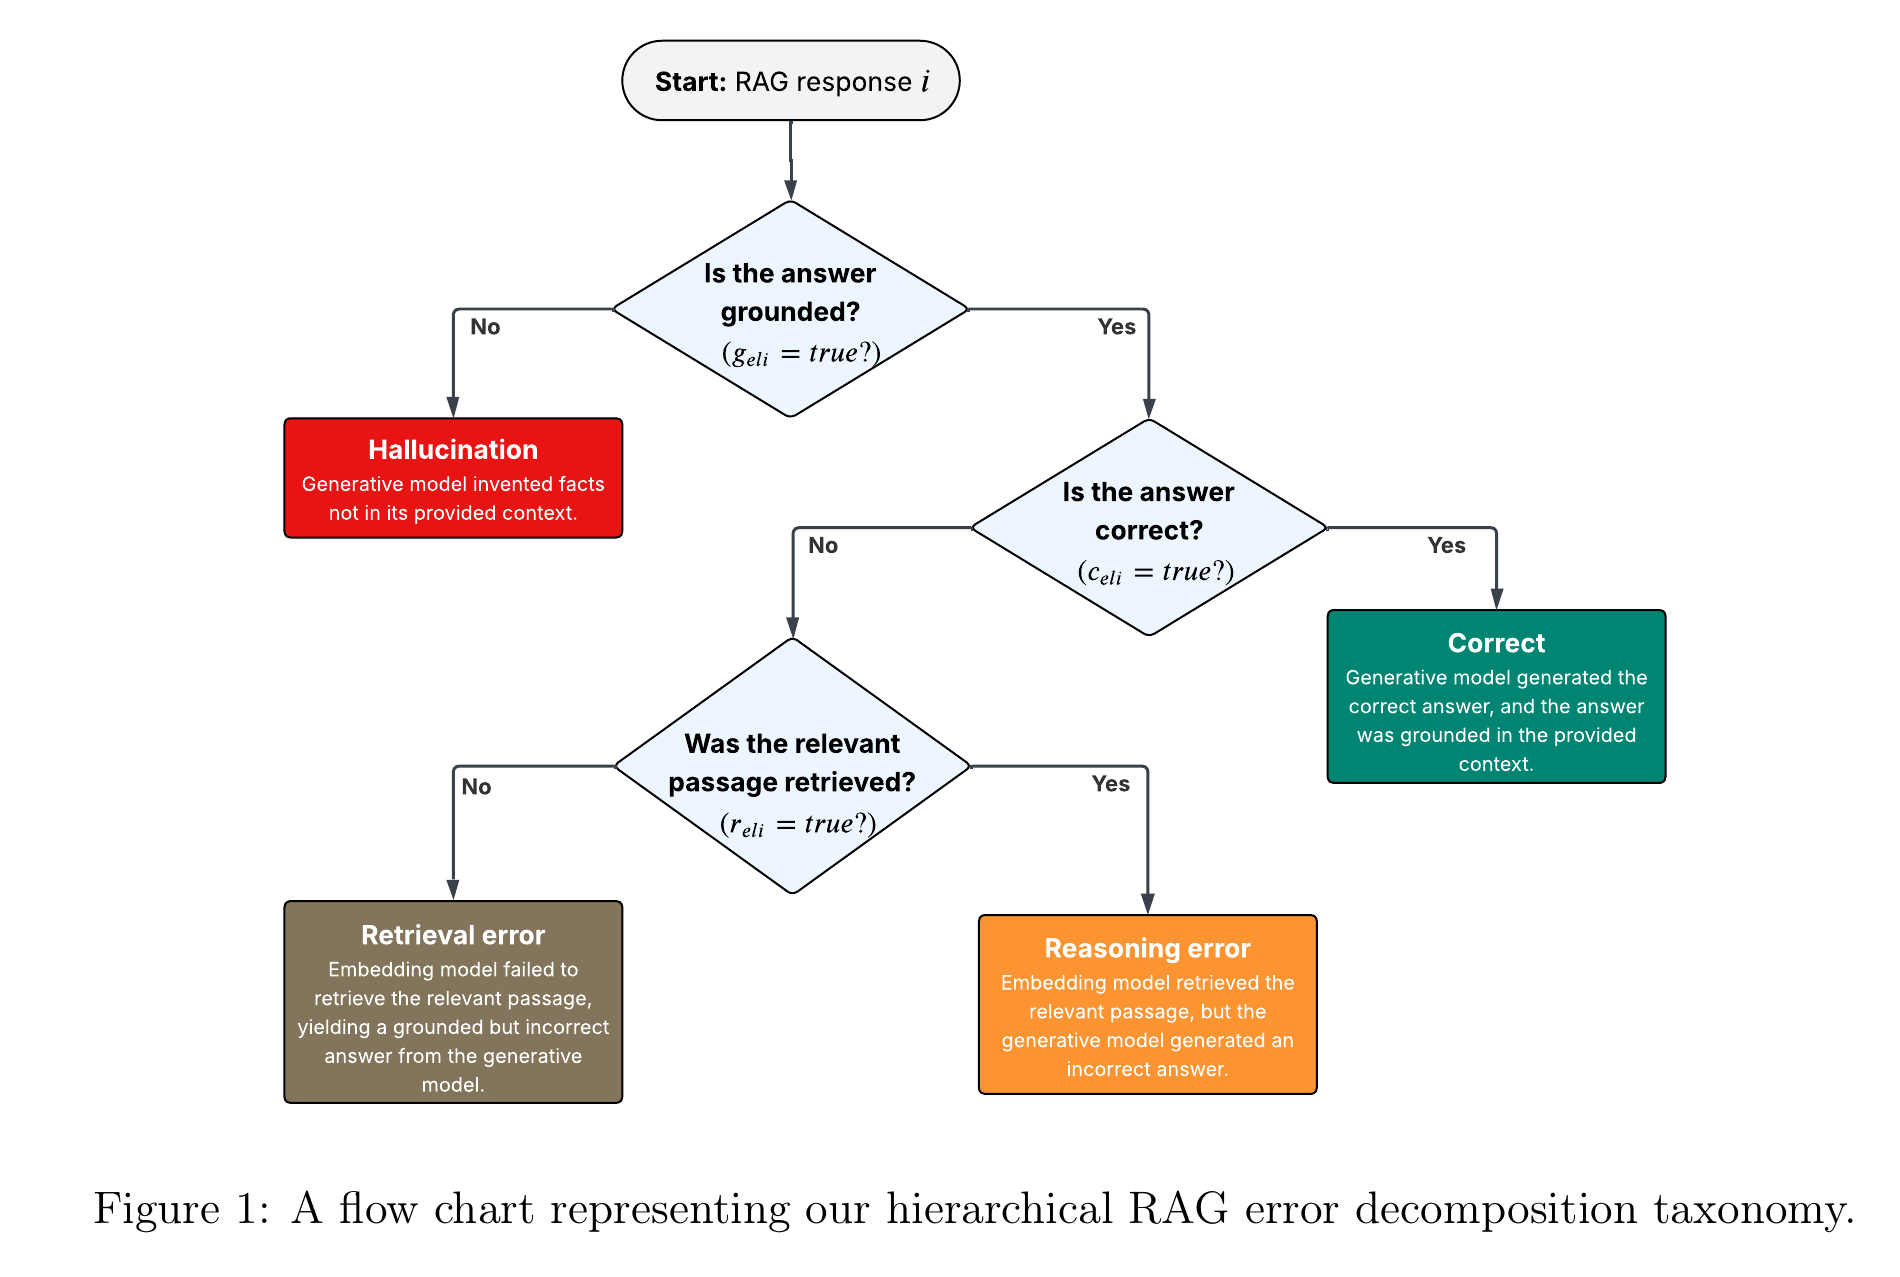
\includegraphics[width=\textwidth]{images/butler2026_fig1.png}
\caption{Figure reproduced from \citet{butler2026}: the hierarchical RAG error-decomposition
taxonomy. Rather than reporting one aggregate accuracy score, the taxonomy separates three
distinct failure modes using three binary signals collected per question, embedding model, and
LLM: groundedness ($g$, whether the answer is supported by what was retrieved), retrieval
accuracy ($r$, whether the annotated supporting passage was actually retrieved), and correctness
($c$, whether the answer entails the reference answer). This distinguishes an ungrounded
hallucination from a grounded answer that is wrong because retrieval failed, and from a grounded,
correctly retrieved answer that the generator still reasoned about incorrectly.}
\label{fig:rag-errors}
\end{figure*}
